\section{Ergebnisse}
\todo{Deadline: 01.07.}
\todo{Noch in Arbeit}
\todo{Sobald wir zuverlässige Ergebnisse produzieren können, mache ich mir hier weiter Gedanken. Es wird aber darauf hinauslaufen, dass ich produzierte Ergebnisse beschreibe und ein paar Diagramme zeige.}


\begin{figure}[H]
	\centering
	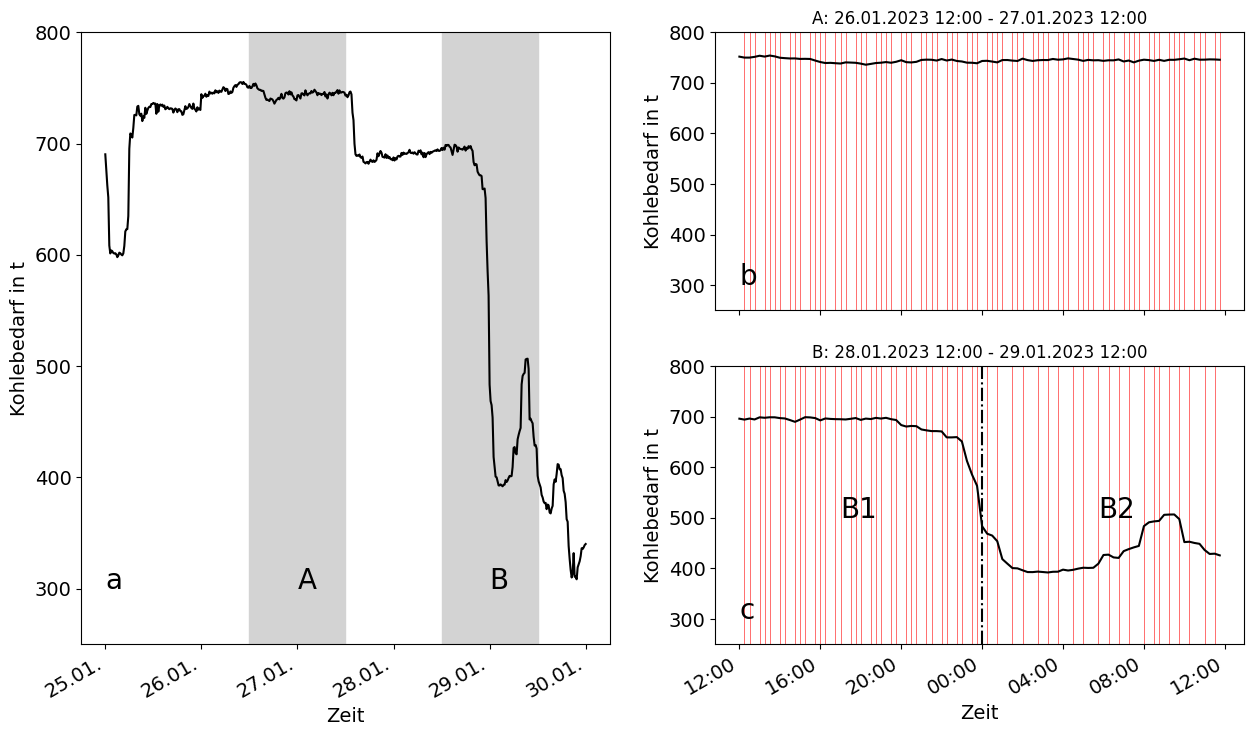
\includegraphics[width=1.0\linewidth]{images/results/departures.png}
	\caption{}
	\label{fig:results-departures}
\end{figure}

\begin{figure}[H]
	\centering
	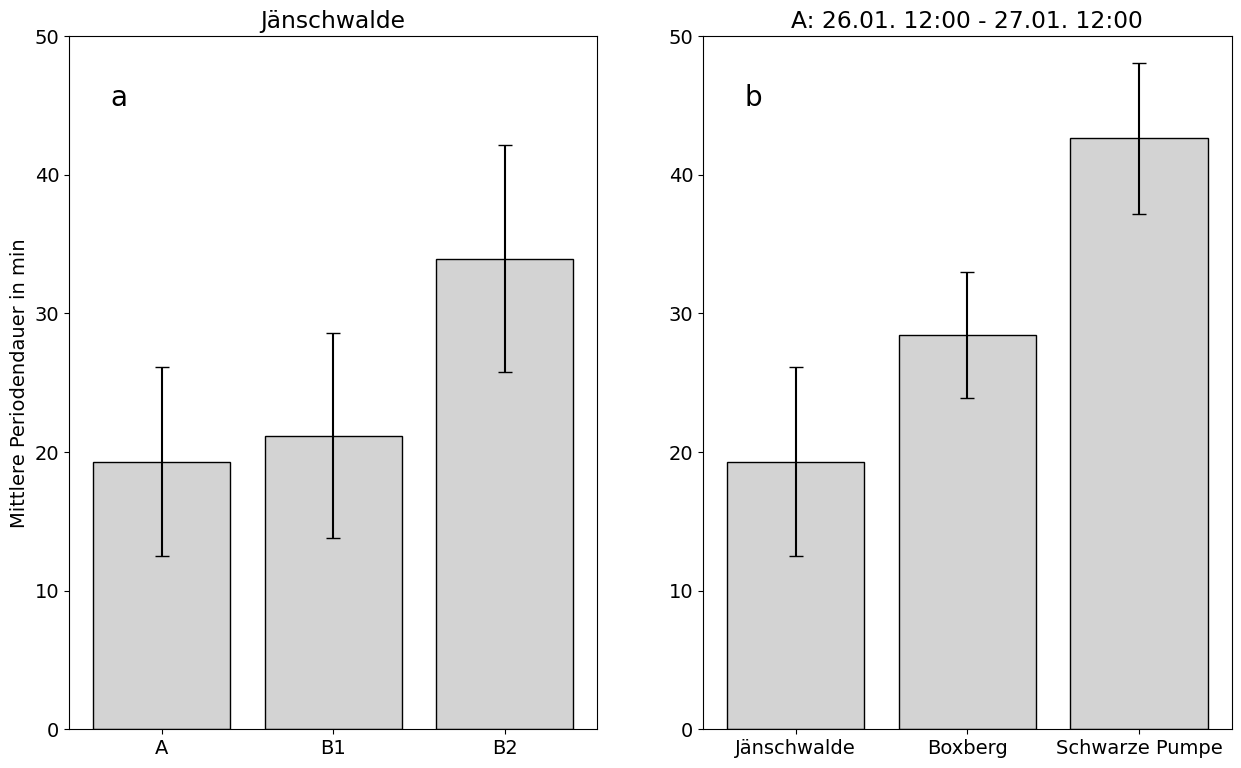
\includegraphics[width=1.0\linewidth]{images/results/periods.png}
	\caption{}
	\label{fig:results-periods}
\end{figure}


\begin{table}[!ht]
	\centering
	\caption{Mittlere Abfahrtsperioden in min für die drei Zeiträume A, B1 und B2 zum Karftwerk Jänschwalde (oberer Tabellenteil) und für die drei Kraftwerke Jänschwalde, Boxberg und Schwarze Pumpe im Zeitraum A (unterer Tabellenteil). Zeitraum A: 26.01. 12:00 - 27.01. 12:00, Zeitraum B1: 28.01. 12:00 - 29.01. 00:00, Zeitraum B2: 29.01. 00:00 - 29.01. 12:00}
	\label{tab:results}
	\begin{tabular}{|l|r|}
		\hline
		\textbf{Zeitraum} & \textbf{Mittlere Abfahrtsperiode in min} \\
		\hline
		\hline
		A & $44,03 \pm 3,69$\\
		\hline
		B1 & $49,00 \pm 8,60$\\
		\hline
        B2 & $75,00 \pm 8,02$\\
		\hline
		\hline
        \textbf{Kraftwerk} & \\
		\hline
		\hline
        Jänschwalde & $44,03 \pm 3,69$\\
		\hline
        Boxberg & $63,57 \pm 6,39$\\
		\hline
		Schwarze Pumpe & $95,36 \pm 7,19$\\
		\hline
	\end{tabular}
\end{table}